\documentclass[letterpaper,11pt]{article}
\usepackage[utf8]{inputenc}
\usepackage[T1]{fontenc}
\usepackage{amsmath}
\usepackage{amssymb}
\usepackage{xcolor}
\usepackage{tikz, float}
\usetikzlibrary{patterns,shapes.misc}

\begin{document}

    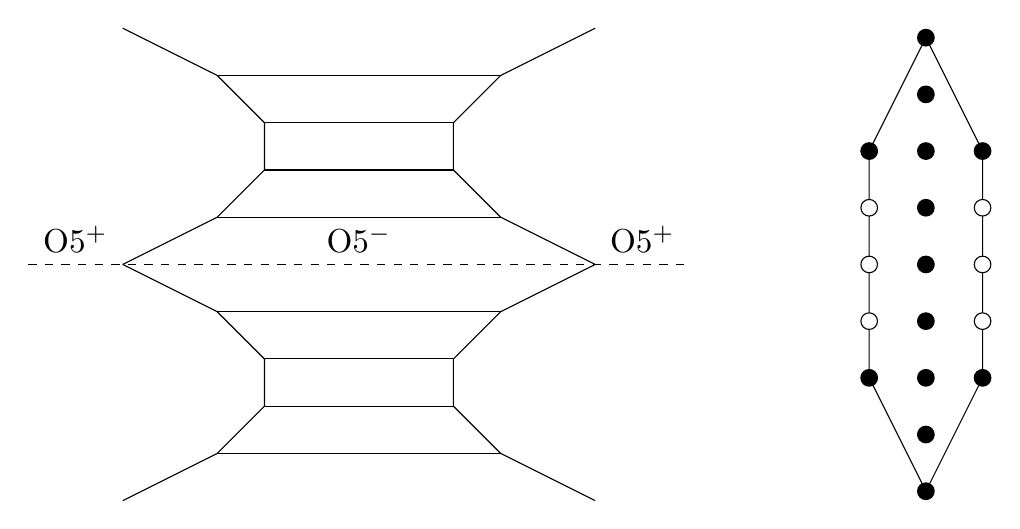
\begin{tikzpicture}[scale=0.6, every node/.style={scale=1.2}]
 \begin{scope}
    \draw[dashed] (-7, 0) -- (7,0);
    \draw (5,0) -- (3,1) -- (2,2) -- (2,3) -- (3,4) -- (5,5) ;
    \draw (-5,0) -- (-3,1) -- (-2,2) -- (-2,3) -- (-3,4) -- (-5,5) ;
    \draw (5,0) -- (3,-1) -- (2,-2) -- (2,-3) -- (3,-4) -- (5,-5) ;
    \draw (-5,0) -- (-3,-1) -- (-2,-2) -- (-2,-3) -- (-3,-4) -- (-5,-5) ;
    \draw (-3,1) -- (3,1);
    \draw (-3,-1) -- (3,-1);
    \draw (2,2) -- (-2,2);
    \draw (2,-2) -- (-2,-2);
    \draw (2,2) -- (-2,2);
    \draw (2,-2) -- (-2,-2);
    \draw (2,3) -- (-2,3);
    \draw (2,-3) -- (-2,-3);
    \draw (3,4) -- (-3,4);
    \draw (3,-4) -- (-3,-4);

    \node[above] at (6,0) {O5$^+$};
    \node[above] at (0,0) {O5$^-$};
    \node[above] at (-6,0) {O5$^+$};
\end{scope}
 \begin{scope}[xshift = 12cm]
 \draw (0, 1.2 * 4) -- (1.2, 1.2 * 2) -- (1.2, - 1.2 * 2) -- (0, - 1.2 * 4) -- (-1.2, - 1.2 * 2) -- (- 1.2, 1.2 * 2)-- (0, 1.2 * 4);
\foreach \i in {-4, -3, ..., 3, 4}
{ \filldraw[] (0, 1.2 * \i) circle (5pt);
}
\foreach \i in {-1, 0, 1}
{ \filldraw[fill=white] (-1.2, 1.2 * \i) circle (5pt);
}
\foreach \i in {-1, 0, 1}
{ \filldraw[fill=white] (1.2, 1.2 * \i) circle (5pt);
}
\filldraw[] (-1.2, 1.2 * 2) circle (5pt);
\filldraw[] (-1.2, -1.2 * 2) circle (5pt);
\filldraw[] (1.2, -1.2 * 2) circle (5pt);
\filldraw[] (1.2, 1.2 * 2) circle (5pt);
\end{scope}
    \end{tikzpicture}

\end{document}